\chapter{AIDA-2020 testbeams}
\label{chapter:aidatestbeams}
 
\epigraph{I love fools' experiments. \\I am always making them.}{Charles Darwin}

One of the most important aspects of testing and developing DQM4hep was to ensure that it was as generic as it was intended to be, and this meant deploying and using the framework on physics testbeams. DQM4hep was originally developed during testbeams of the \acrfull{siwecal}, and its early testing phases were predominantly based on this detector, so it was apparent that it could be used in the originally-intended setting. However, in trying to develop it as a generic monitor, and to satisfy the requirements of a generic data monitoring and quality monitoring tool for AIDA-2020, it was essential that it was tested on other detectors of different types to demonstrate its generic nature. 

In this chapter, deployment, testing and usage of DQM4hep on testbeams within the AIDA-2020 collaboration will be discussed in detail. For a testbeam where DQM4hep was deployed outside of the AIDA-2020 community, see Chapter \ref{chapter:ideatestbeam}. Three testbeams will be described in detail, as they represent the different stages of using DQM4hep as a data monitoring tool, from first implementation and deployment, to further developments, and finally as a mature tool.

\section{Introduction}
The CALICE testbeams were done within the \textit{Forschung mit Lepton Collidern}\footnote{``Research with lepton colliders'' in English} group (FLC) based at DESY in Hamburg, working on the \acrfull{ahcal} prototype during its development. Regular testbeams were held at the DESY II synchrotron at \acrshort{desy} in Hamburg, Germany and at the \acrfull{sps} at CERN in Geneva, Switzerland. The goals for these testbeams varied over time but common focuses for the hardware were power-pulsing tests, and commissioning and calibration of new detector boards to test variations and changes to the manufacturing process. The testbeams were often used as testbeds for data acquisition electronics and software, such as the \acrshort{eudaq} data acquisition software, the \acrshort{bif} device, and DQM4hep.

DQM4hep was used as an online monitoring and data quality monitoring tool for \acrshort{ahcal} tesbeams beginning in May 2016, and in further testbeams between 2016 and 2018. The majority of these testbeams occurred at the DESY II facility, but two took place at the CERN SPS in May 2017 and June 2018.

\subsection*{The AHCAL prototype} % Full dossier on the AHCAL here: https://iopscience.iop.org/article/10.1088/1748-0221/5/05/P05004/pdf
The \acrfull{ahcal} is a sampling calorimeter formed of steel absorber plates and plastic scintillator tiles, read out by silicon photomultipliers (\acrshort{sipm}s) as active material\cite{proceedings-ahcal-prototype}. One of the important features of the AHCAL is that the prototypes were designed to be made using techniques suitible for mass production, such as injection-moulding and automated foil-wrapping of the scintillator tiles, and pick-and-place assembly of the layers and their electronics. It also uses power pulsing -- rapidly cycling power so that the electronics are active only when the beam is present, according to a known beam structure. This helps to reduce power consumption and head production, making cooling the layers easier.

\section{May 2016 at DESY II}
The first deployment of DQM4hep on an AHCAL testbeam was at DESY II during May 2016. The testbeam was to be two weeks in duration, following a one-week setup and preparation period. Besides testing the deployment and usage of DQM4hep, the goals of this testbeam where to test \acrshort{mip} calibration of a new AHCAL base unit (HBU), to test the power pulsing feature, and to perform \acrshort{tdc} calibrations. In addition to these goals for the AHCAL, a device called a \acrfull{bif}, another part of the ongoing work of AIDA-2020 Work Package 5, was being tested. % Reference something for this - wiki pages are here (http://flcwiki.desy.de/AHCALandBIF_TestBeamDESYMay2016) but ideally we want a report.

Before and during the testbeam, the majority of the development for AHCAL-specific analysis modules was undertaken. Prior to this, DQM4hep had only been used on SiWECAL beams, and was untested for other detectors. 

File reader and streamer plugins for the LCIO data format were already available in the now-deprecated \texttt{dqm4ilc} package, which meant that the framework could open and access the data format already.

\subsection{Data format}
The data for the AHCAL is in the \acrfull{lcio} format, using an object type called LCGenericObject, which is a generic format for use when the existing data formats are not suitable. It comprises two parts: the block of data itself, held in 14-bit numbers; and a header containing user-defined parameters, in this case a timestamp, a typename for the object, and a description of the data contained in the object.

The structure of a single event in LCGenericObject format can be seen below, which is the result of using the \texttt{dumpevent} tool to dump the contents of an LCIO event to the command line:

% Really we should be using a file from the May 2016 testbeam here, just for consistency
\begin{verbatim}
--------------- print out of LCGenericObject collection --------------- 

  flag:  0x0
 parameter DAQquality [int]: 1, 
 parameter DataDescription [string]: i:CycleNr,i:BunchXID,i:EvtNr,i:ChipID,
     i:NChannels,i:TDC14bit[NC],i:ADC14bit[NC], 
 parameter Timestamp [string]: Thu, 25 May 2017 05:38:25 +0200, 
 parameter TypeName [string]: CaliceObject, 

 [   id   ] i:Type,i:EventCnt,i:TS_Low,i:TS_High - isFixedSize: false
 --------------------------------------------------------
 [00000852] i:99; i:0; i:0; i:121; i:36; i:13365; i:13383; i:13378; i:13370;
     i:13336; i:13351; i:13361; i:13365; i:13357; i:13338; i:13345; i:13368;
     i:13386; i:13380; i:13386; i:13391; i:13382; i:13363; i:13395; i:13342;
     i:13378; i:13335; i:13327; i:13376; i:13342; i:13373; i:13406; i:13323;
     i:13361; i:13395; i:13378; i:13365; i:13362; i:13378; i:13384; i:13355;
     i:12288; i:12288; i:12288; i:12288; i:12288; i:12288; i:12288; i:12288;
     i:12288; i:12288; i:12288; i:12288; i:12288; i:12288; i:12288; i:12288;
     i:12288; i:12288; i:12288; i:12288; i:12288; i:12288; i:12288; i:12288;
     i:12288; i:12288; i:12288; i:12288; i:12288; i:12288; i:12288; i:12288;
     i:12288; i:12288; i:12288; i:12288;
 --------------------------------------------------------
\end{verbatim}

In this case, the \texttt{TDC14bit[NC]} and \texttt{ADC14bit[NC]} are arrays, each holding a number of elements equal to the \texttt{NChannels} variable, in this case 36. Each element of these arrays corresponds to a single physical scintillator tile within the detector, and identifies which chip it belongs to using \texttt{ChipID}. 

The \texttt{ADC14bit} and \texttt{TDC14bit} arrays contain binary data, which is represented above converted directly to decimal. However some bits represent data other than the actual ADC or TDC, such as validation bits, hit bits, etc. An explanation of the structure of these bits can be seen in [ref]. % Need to find the bit structure, maybe on a presentation Adrian gave?

[...]

\subsection{Results}
Over the course of the preparation week, the foundations were laid for the analysis module. This involved gaining a familiarity with the data structure, loading data from previous testbeams into DQM4hep offline, and attempting to read it in basic ways. The first module was not ready for the beginning of the testbeam proper, but a few days afterwards we were able to produce plots in DQM4hep from ``nearly-online'' testbeam data.

The first analysis module developed was the \texttt{AHCALRawModule}. The majority of the processing in this module was decoding of the data from the binary format and extracting the information from it. After this, validation bits and hit bits in the data were checked to classify data as `good' or `bad' hits. Then the actual ADCs and TDCs were filled into their respective histograms. 

The first module acted as a proof-of-concept, and once this was done further work started on creating more modules with a wider variety of features and plots to provide better coverage for online monitoring. We created and refined two separate modules during this testbeam -- \texttt{AHCALRawModuleChannel} and \texttt{AHCALRawModuleGlobal}. 

The channel module created a per-spectrum channel of all ADCs, integrated over the whole run. It was able to load a number of individual channels, though due to the memory requirement, it could not track all channels simultaneously. To work around this, we implemented a facility for the module to read which channels to monitor from the XML steering file, so that these could be defined at runtime. An example of some of the per-channel spectra created using this module can be seen in Fig. \ref{figure:aida/may2016/channelmodule}

The global module produced a 2D histogram containing cells for each channel, coloured for the \acrshort{adc} in that channel. This didn't produce a hitmap as the geometry information was not available in this plot, but did allow easy identification of dead channels and channels that were in the beamspot. An example of this can be seen in Fig. \ref{figure:aida/may2016/globalmodule}.

\begin{figure}[p]
	\centering
	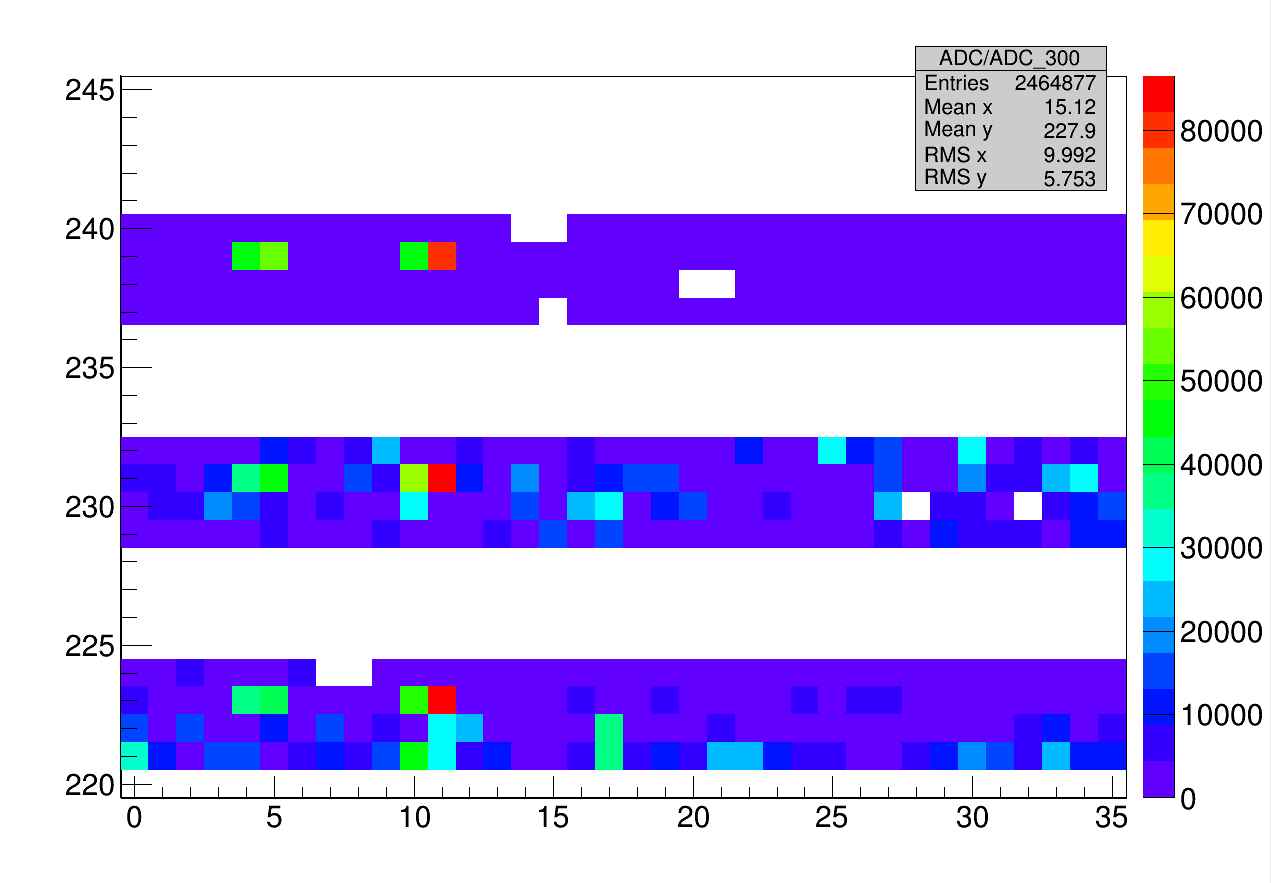
\includegraphics[width=0.85\textwidth]{../Pictures/GlobalModule-May2016.png} % Add axis labels: x is channel no., y is ChipID
	\caption{Histogram produced by \texttt{AHCALRawModuleGlobal} showing all ADCs exceeding 300 over a single run. Dead or nonresponsive channels are seen as white squares. The horizontal gaps are due to the fact that some ChipIDs were not present.}
	\label{figure:aida/may2016/globalmodule}
\end{figure}

\begin{figure}[p]
	\centering
	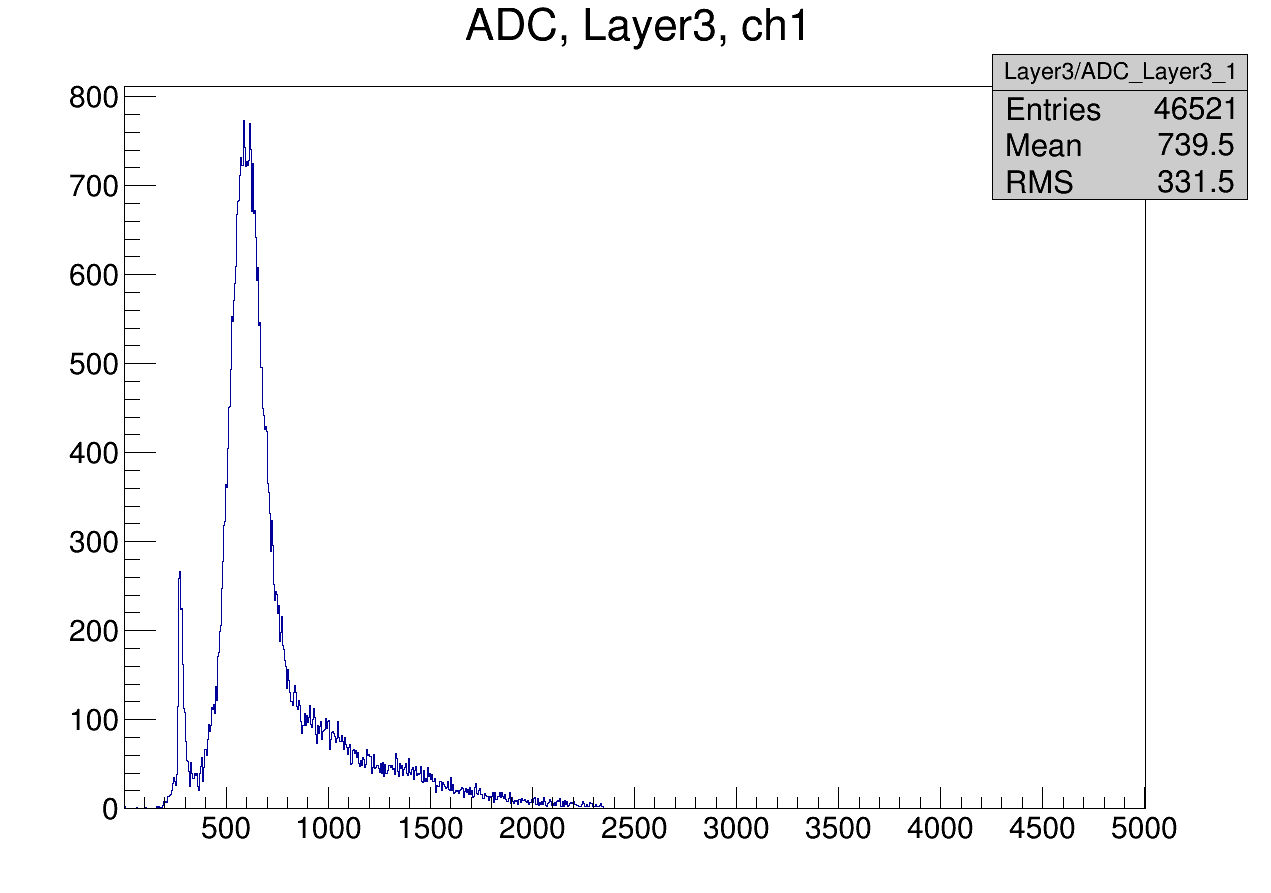
\includegraphics[width=0.95\textwidth]{../Pictures/ChannelModule-May2016.png} % Add an x-axis label to this too
	\caption{Histogram produced by \texttt{AHCALRawModuleChannel} showing an ADC spectrum for a single run. The pedestal can be seen at ~300 and the MIP peak at ~650.}
	\label{figure:aida/may2016/channelmodule}
\end{figure}

[...] % Text here talking about monitoring overall.

\begin{figure}
	\centering
	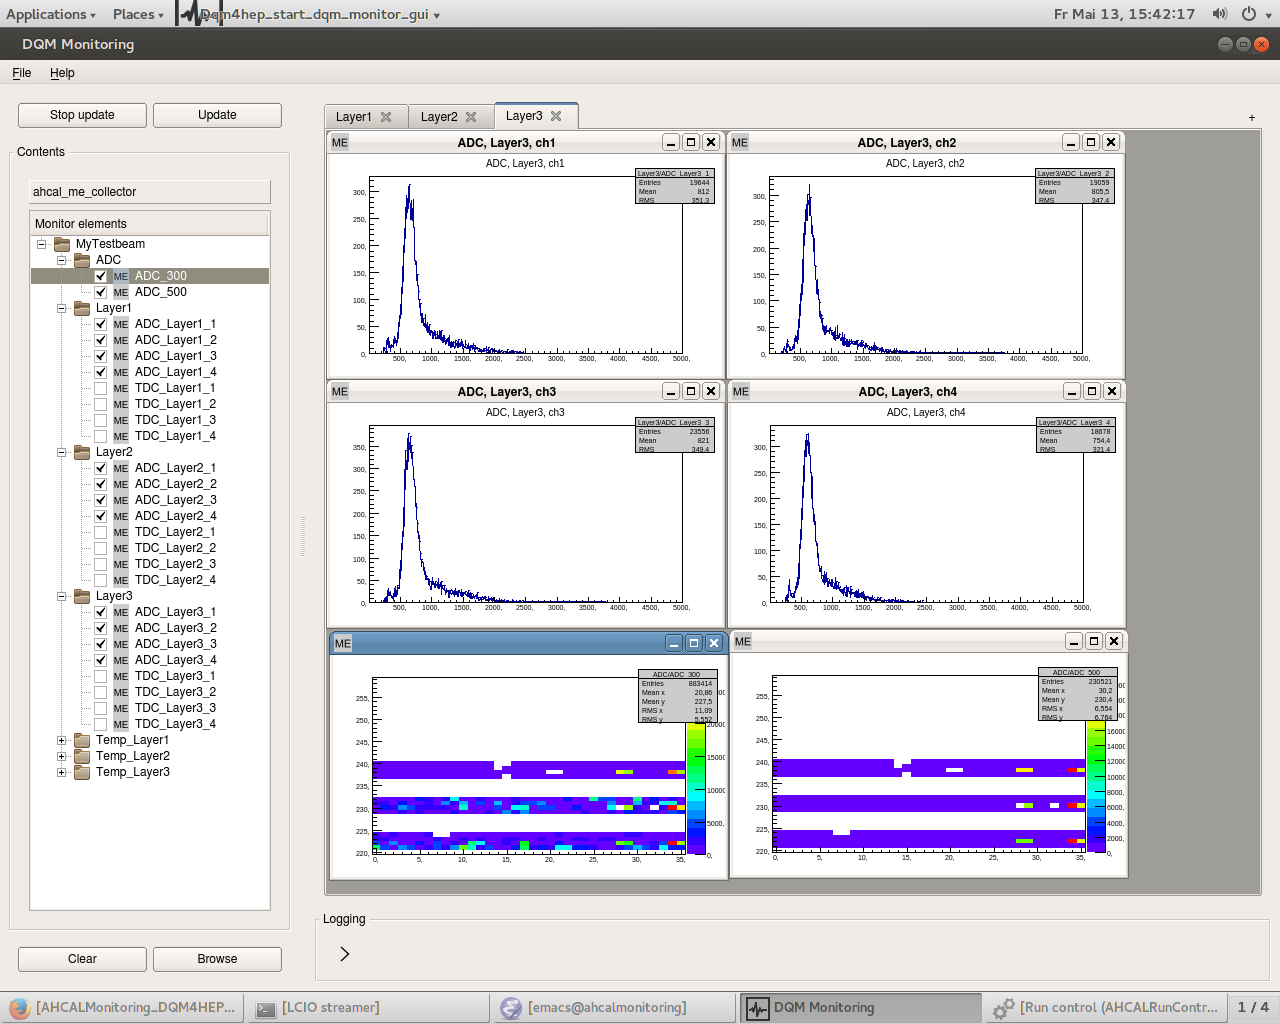
\includegraphics[width=0.95\textwidth]{../Pictures/PowerPulsingMipScans-May2016.png}
	\caption{A full screencapture from the May 2016 testbeam showing the monitoring interface in use during power pulsing tests, displaying a MIP scan.}
	\label{figure:aida/may2016/overview}
\end{figure}

\section{July 2016 DESY II}
The next usage of DQM4hep was a testbeam also at DESY II during July 2016. The testbeam was to be one week long, with a one-week preparation period. The primary goal for DQM4hep in this testbeam was to establish hitmaps of the calorimeter. This would give a visual representation of the layers, allowing identification of the beamspot, allowing dead or mis-calibrated channels to be identified visually, as well as to monitor [...]

Creating a hitmap for the AHCAL was nontrivial, as the information coming from the data acquisition device and stored in LCIO format did not encode location. Each channel was instead identified by its ``electronics number'' -- a combination of the ChipID of the board the channel was located on, and the number of the channel on that board.

Each layer was formed of four boards (each one with a ChipID), each of which contained sixteen layers. The orientation of the boards, which boards were in a layer, and the order of the layers in the stack were all changeable, so an additional requirement for the hitmap function was that it could take an external geometry file that could be changed or automatically generated. 

DQM4hep has internal functions for parsing XML data into internal structures, so an XML file was chosen as the format to store the geometry data. By making this an XML file, it avoided hard-coding the geometry into the framework itself, allowing the geometry data to be changed at runtime. The AHCAL team also already had an internal format for the geometry file used for offline processing after testbeams, which could be converted into the XML format via a shell script.

For analysis modules needing geometry, the XML file wasgiven as a required parameter for the steering file, which then built a C++ map of the correspondence between electronics number and $(i,j,k)$ co-ordinates of each channel in memory during initialisation. Then a function called \texttt{electronicsToIJK} was written that took the electronics number as the argument and returned the position of the channel in geometric co-ordinates. A further function was written, called \texttt{IJKToElectronics}, that performed the opposite operation, but this was not used. 

Using these new functions, another analysismodule called \texttt{AHCALHitmap} was written that created a two dimensional histogram, with each bin representing a channel on the $x$ and $y$ axes for a single layer. This histogram was then filled with with the ADCs of that channel for the whole event, producing a hitmap.

\subsection{Results}
[...]

\section{December 2016 at DESY II} % There was also one in October, which I can't remember if I went to or not.
[...]

\section{May 2017 at CERN SPS} % Wiki pages are here (http://flcwiki.desy.de/AHCALTestBeamCERN2017) but we ideally want an actual report for this.

During May 2017, testbeam time at CERN's Super Proton Synchrotron (SPS) facility was used for further tests for the AHCAL.

\begin{center}
	[Figure: we have plenty of pictures of the testbeam area and the installation.]
\end{center}

[...]

During this testbeam, the analysis modules had become mature, and represented the majority of the needed online monitoring for the testbeam, especially because the data format of the detector had been fixed for some time. Because of this, after the initial set-up and verification stages, very little management or editing of the monitoring software was necessary. It was instead used as intended -- a tool for shifters to use to troubleshoot problems with the beam or detectors. It was successfully used to identify dead channels on several of the boards [confirm this].

[...]

\subsection{Results}
[...]

\begin{center}
	[Plots from the AHCAL CERN testbeam]
\end{center}
